%%%%%%%%%%%%%%%%%%%%%%%%%%%%%%%%%%%%%%%%%%%%%%%%%%%%%%%%%%%%%%%%%%%%%%%%%%%%%%%
%% Dokumentation für Praxisprojekt                                           %%
%% (TH Köln -Campus Gummersbach, Fak. 10)                                    %%
%%                                                                           %% %%
%% LIZENZ:                                                                   %%
%% Diese Vorlage darf nicht kommerziell verbreitet                           %%
%% werden. Eine nicht-kommerzielle Weitergabe ist                            %% 
%% gestattet.                                                                %%
%%                                                                           %%
%% Von Ludger Schönfeld, M. Sc.,
%% 2014-2017                            %%
%%%%%%%%%%%%%%%%%%%%%%%%%%%%%%%%%%%%%%%%%%%%%%%%%%%%%%%%%%%%%%%%%%%%%%%%%%%%%%%

%%%%%%%%%%%%%%%%%%%%%%%%%%%%%%%%%%%%%%%%%%%%%
%% HEADER                                  %%
%%%%%%%%%%%%%%%%%%%%%%%%%%%%%%%%%%%%%%%%%%%%%
\documentclass[a4paper,12pt,oneside]{article}
% Optionen:
% - a4paper => DIN A4-Format
% - 12pt    => Schriftgröße (weitere  
%              grundlegende Fontgrößen: 10pt, 11pt)
% - oneside => Einseitiger Druck

%% Verwendete Pakete:
\usepackage[ngerman]{babel} % für die deutsche Sprache
\usepackage{caption} % Für schönere Bildunterschriften
\usepackage[T1]{fontenc} % Schriftkodierung (Für Sonderzeichen u.a.)
\usepackage[utf8]{inputenc} % Für die direkte Eingabe von Umlauten im Editor u.a.
\usepackage{fancyhdr} % Für Kopf- und Fußzeilen
\usepackage{lscape} % Für Querformat
\usepackage{hyperref} % Für Hyperlinks


%% Show code in a better way
\usepackage{listings}
\usepackage{color}

\definecolor{dkgreen}{rgb}{0,0.6,0}
\definecolor{gray}{rgb}{0.5,0.5,0.5}
\definecolor{mauve}{rgb}{0.58,0,0.82}

\lstset{frame=tb,
  language=Java,
  aboveskip=3mm,
  belowskip=3mm,
  showstringspaces=false,
  columns=flexible,
  basicstyle={\small\ttfamily},
  numbers=none,
  numberstyle=\tiny\color{gray},
  keywordstyle=\color{blue},
  commentstyle=\color{dkgreen},
  stringstyle=\color{mauve},
  breaklines=true,
  breakatwhitespace=true,
  tabsize=3
}
%% Schriften (Beispiele)
%% Weitere LaTeX-Schriften im "LaTeX Font Catalogue"
%% unter: http://www.tug.dk/FontCatalogue/.
%% ACHTUNG: Ggf. müssen Schriften noch installiert 
%% werden!

% Serifen-Schriften:
\usepackage{lmodern} % Schriftart "Latin Modern"
%\usepackage{garamond} % Schriftart "Garamond"

%Sans Serif-Schriften:
%\usepackage[scaled]{uarial}
%\usepackage[scaled]{helvet}
%%--------------
\usepackage[normalem]{ulem} % Für das Unterstreichen von Text z.B. mit \uline{}
\usepackage[left=3cm,right=2cm,top=1.5cm,bottom=1cm,
textheight=245mm,textwidth=160mm,includeheadfoot,headsep=1cm,
footskip=1cm,headheight=14.599pt]{geometry} % Einrichtung der Seite 

\usepackage{graphicx} % Zum Laden von Graphiken
\graphicspath{ {./sources/} }

% INFO: Graphiken einbinden
%
% \includegraphics[scale=1.00]{dateiname}
%
% => Ausgabeformat: PDF-Dokument:
%    Es können die folgenden (Graphik-)formate eingebunden
%    werden: .jpg, .png, .pdf, .mps
% 
% => Ausgabeformat: DVI/PS:
%    Folgende (Graphik-)formate werden unterstützt:
%    .eps, .ps, .bmp, .pict, .pntg
\usepackage{epstopdf}

% Pakete für Tabellen
\usepackage{tabularx} % Einfache Tabellen
\usepackage{longtable} % Tabellen als Gleitobjekte (für die Aufteilung bei langen 
 %Tabellen über mehrere Seiten)
\usepackage{multirow} % Für das Verbinden von Zeilen innerhalb einer Tabelle mit
 % \multirow{anzahl}{*}{Text}

% (Zusatz-)Pakete für Formeln
\usepackage{amsmath}
\usepackage{amsthm}
\usepackage{amsfonts}

\usepackage{setspace} % Paket zum Setzen des Zeilenabstandes
% INFO: Zeilenabstand setzen:
%
% Befehle:
% - \singlespacing  => 1-zeilig (Standard)
% - \onehalfspacing => 1,5-zeilig
% - \doublespacing  => 2-zeilig 
\onehalfspacing % Zeilenabstand auf 1,5-zeilig setzen

% Farbboxen (für die Merkkästen in dieser Vorlage):
\usepackage{tcolorbox}
\tcbset{colback=white,colframe=orange,
        fonttitle=\bfseries}

\usepackage[colorlinks,pdfpagelabels,pdfstartview=FitH,
bookmarksopen=true,bookmarksnumbered=true,linkcolor=black,
plainpages=false,hypertexnames=false,citecolor=black]{hyperref} % Für Verlinkungen
% INFO: Verlinkungen mit dem hyperref-Paket:
%
% Die Angabe von URLs mit dem Befehl \url{} erlaubt einen
% gesonderten Umgang mit Weblinks. Denn die Links werden verlinkt.
% Auch erfolgt automatisch am Zeilenende ein Umbruch des Links.
% Es ist auch nicht erforderlich, Sonderzeichen in der URL manuell zu 
% entschärfen.
%
% TIPP: Sollte ein Umbuch bei einem Link nicht automatisch erfolgen, so kann
% das daran liegen, dass ein/mehrere Zeichen zusätzlich angegeben werden müssen,
% an dem der Link umbrochen werden kann.
% Dies kann mit folgendem Befehl erfolgen (Beispiel):
% \renewcommand*\UrlBreaks{\do-\do_}

% Das Paket "biblatex" für autom. 
% Literaturverzeichnisse:
%\usepackage{csquotes} % Für sprachangepasste Anführungszeichen
%\usepackage[backend=bibtex,style=alphabetic]  
%           {biblatex}
%\addbibresource{bib/literatur.bib}           

%%%%%%%%%%%%%%%%%%%%%%%%%%%%%%%%%%%%%%%%%%%%%
%% DOKUMENT                                %%
%%%%%%%%%%%%%%%%%%%%%%%%%%%%%%%%%%%%%%%%%%%%%

\begin{document}
% Unbeschriftetes Vorblatt (Leere Seite)
\pagestyle{empty} % Seite ohne Kopf- und Fußzeilen
\newpage % Neue Seite
\input{leereSeite} % Ausgelagerte LaTeX-Datei (hier: leereSeite.tex) einbinden

\newpage

% Deckblatt
\pagestyle{empty}
\begin{titlepage}
  
\includegraphics[scale=0.20]{sources/TH_Koeln_Logo}\\
  \begin{center}
    \Large
    Technische Hochschule Köln\\
    Fakultät für Informatik und Ingenieurwissenschaften\\
    \hrule\par\rule{0pt}{2cm} % Horizontale Trennlinie  mit 2 cm Abtand nach unten erzeugen
    \LARGE
    \textsc{BERICHT ZUM PRAXISPROJEKT}\\
    \vspace{1cm} % Vertikaler Abstand von 1cm erzeugen
    \huge
    Plattform für die Spielersuche\\
    \Large
    Eine mit Javascript entwickelte Plattform\\
    \vspace{1cm}
    \large
    Vorgelegt an der TH Köln Campus Gummersbach\\
    im Studiengang Wirtshaftsinformatik\\
    \vspace{1.0cm}
    ausgearbeitet von:\\
    \textsc{Timo Kalter} 12345678\\
    \textsc{Carlo Menjivar} 11117929\\
    \vspace{1cm}
    \begin{tabular}{ll} % Einfache Tabelle ohne Rahmen, mit 2 Spalten erzeugen
      \textbf{Erster Prüfer:}  & Frau Prof. Birgit Bertelsmeier \\
      \textbf{Zweiter Prüfer:} & <Name des 2. Prüfers> \\
    \end{tabular}
    \vspace{1cm}
    \\Gummersbach, im <Monat der Abgabe>
  \end{center}
\end{titlepage}

\newpage

% Abstract (ACHTUNG: Abweichung zur Reihenfolge im Merkblatt!)
\begin{abstract}
  Platz für das deutsche Abstract...
\end{abstract}

\renewcommand{\abstractname}{Abstract}
\begin{abstract}
  Platz für das englische Abstract...
\end{abstract}
%<MERKKASTEN> (für die eigene Verwendung bitte entfernen
\vspace{1cm}
\begin{tcolorbox}[title={Das Abstract}]
  Bei einem Abstract handelt es sich um eine Art \textit{Zusammenfassung} Ihrer Arbeit. Diese kann in deutscher und/oder englischer Sprache verfasst werden. Mithilfe des Abstracts kann der Leser sich zügig orientieren, in wie fern Ihre Arbeit für ihn Relevanz besitzt.\\                                                                      Sprechen Sie unbedingt mit Ihrer Betreuerin/Ihrem Betreuer, ob Sie für Ihre Arbeit ein Abstract benötigen.\\
  Ein Abstract beinhaltet folgende Aspekte \footnote{ Vgl. \cite{SW11}, S. 249}:
  \begin{itemize}
    \item Ziel der Arbeit
    \item Fragestellung der Arbeit
    \item Herangezogener, theoretischer Ansatz ("Quellen")
    \item \textit{Optional:} Methodik
  \end{itemize}
\end{tcolorbox}
%</MERKKASTEN>

%<MERKKASTEN> (für die eigene Verwendung bitte entfernen
\vspace{1cm}
\begin{tcolorbox}[title={Hinweise zu dieser Dokumentvorlage}]
  \begin{itemize}
    \item Es handelt sich hierbei um eine Beispiel-Vorlage für wissenschaftliche Ausarbeitungen.
          Über die konkrete, formale Ausgestaltung Ihrer wissenschaftlichen Arbeit sprechen Sie unbedingt mit Ihre/m Betreuer/in.
    \item Unabhängig, ob Sie beispielsweise eine Bachelor-, Master- oder Hausarbeit schreiben müssen. Diese Vorlage kann als eine gute Basis für Ihre Arbeit dienen. Passen Sie einfach die Vorlage Ihren Anforderungen entsprechend an.
  \end{itemize}
\end{tcolorbox}
%</MERKKASTEN>

\newpage

% Inhaltsverzeichnis
\tableofcontents

\newpage
\pagestyle{fancy} % Kopf- und Fußzeilen aktivieren (=> Paket "fancyhdr")

% Abbildungsverzeichnis
% INFO: Abbildung einbinden (Beispiel):
%  \begin{figure}[h!]
%    \centering
%    \includegraphics[scale=1.00]{Pfad zum Bild}\\
%    \caption{Bildunterschrift}
%    \label{Marke zum Referenzieren auf die Abbildung}
%  \end{figure}
\section*{Abbildungsverzeichnis}
\addcontentsline{toc}{section}{Abbildungsverzeichnis} % Manuellen Eintrag im Inhaltsverzeichnis erzeugen
\renewcommand{\listfigurename}{} % Name des Abbildungsverzeichnisses ändern
\thispagestyle{empty}
\listoffigures

\newpage

% Tabellenverzeichnis
%\addcontentsline{toc}{section}{Tabellenverzeichnis}
%\listoftables

%\newpage

% Hauptteil des Dokuments
% TIPP: Jedes Kapitel oder jeder Abschnitt in eine eigene
% LaTeX-Datei (.tex) auslagern.
% Einbinden der ausgelagerten Dateien in diese Hauptdatei, erfolgt
% mittels folgendem Befehl (Beispiel):
% beispiel.tex => \input{beispiel}
\newpage
% INFO: Querverweise auf Gliederungselemente, Abbildungen
%       & Tabellen setzen:
%
% Voraussetzung: Gesetzte Referenzmarke mit dem Befehl: \label{marke}
%
% Referenzierung erfolgt dann mittels dem Befehl:
% \ref{marke}

\section{Problemstellung}\label{kap_problemstellung}
% Was ist das Problem
\paragraph{}
-- Warum Plattform? --

\paragraph{}
Unsere Aufgabe ist es, eine Webplattform zu erschaffen, die es Nutzern ermöglicht, mit anderen Nutzern in Kontakt zu treten und sich im Chat näher kennenzulernen – mit Fokus auf das gemeinsame Spielen von „League of Legends“. Um dies zu erreichen, sind verschiedene Dinge nötig.

\paragraph{}
Nutzer sollen ein Benutzerkonto anlegen können. Auf dem Profil können sie Informationen von sich preisgeben: Name, Alter, einen Freitext, ein Profilbild, sowie präferierte Rollen im Videospiel. Um neue Kontakte kennenzulernen, soll der Nutzer andere Nutzer „mögen“ können. Dazu gibt es eine spezielle Suchfunktion, bei der zufällige andere Nutzer angezeigt werden. In der Suchfunktion ist es möglich, seine Suche mit Filtern einzugrenzen, um nur bestimmte Nutzergruppen zu zeigen.

\paragraph{}
Nutzer erfahren nicht, wer sie mag. Stattdessen werden andere Nutzer, die sie mögen, bei der Suche weiter vorne angezeigt. Wenn beide Nutzer sich gegenseitig mögen, werden sie Freunde und können in Zukunft miteinander kommunizieren.

\paragraph{}
Wie bei jeder Online-Community wird es Nutzer geben, die durch Fehlverhalten negativ auffallen. Es soll Nutzern möglich sein, diese zu blockieren oder sogar zu melden. Im Falle einer Meldung soll der Nutzer besonders unter die Lupe genommen werden und entsprechend mit ihm verfahren werden – bis zur permanenten Sperrung des Nutzerkontos.

\paragraph{}
Benutzer sollen in der Lage sein, Einstellungen zu verwalten – zum Beispiel, ob und wie sie über neue Nachrichten / „Matches“ erfahren sollen. In den Einstellungen sollen sie zudem ihren Account löschen können.

\paragraph{}
Um Nutzer für unsere Plattform zu gewinnen, soll es eine ansprechende Startseite geben, die dem Nutzer ein Bild von unserer Webseite gibt.

\newpage
\section{Einleitung}\label{kap_einleitung}
WORK IN PROGRESS...

\subsection{Einführung in das Thema (Motivation, zentrale Begriffe etc.)}
\subsection{Hinführung zu den Ergebnissen}
\subsection{Ggf. Angabe des Schwerpunktes}
\subsection{Ggf. Einschränkungen darlegen}
\subsection{Problemstellung}
\subsection{Zielstellung der Arbeit}
\subsection{Fragestellung der Arbeit}

\subsection{Struktur der Arbeit}
Dieser Projektbericht ist in folgenden Kapitel unterteilt:
\textbf{Kapitel 2}
\\\\
\textbf{Kapitel 3}
\\\\
%Frontend
\textbf{Kapitel 4?} erläutert, welche JavaScript-Frameworks zu Beginn des Projekts berücksichtigt wurden. Er gibt einen Überblick über die Faktoren, die zu beachten sind, wenn man sich für React entscheidet, und zeigt schließlich, wie die Daten mit Hilfe der React JavaScript-Bibliothek und ihrer Hooks für den Endbenutzer visualisiert werden.
\\\\
%Serverabfragen 
\textbf{Kapitel 5?} geht es um die Interaktion zwischen dem Client und dem Server. 
\\\\
Anhand von zwei Beispielen wird gezeigt, wie Lese- und Schreibabfragen mit Hilfe von GraphQL und ApolloClient durchgeführt wurden.
\\\\
%Qualitätssicherung
\textbf{Kapitel 6?} zeigt die Relevanz von Testfällen. Sie zeigt auch die Vorteile automatisierter und eingebetteter Testfällen in der Entwicklungsumgebung.
\\

\vspace{1cm}
\begin{tcolorbox}[title={Die Einleitung(DELETE AFTER CHECK WE COMPLETE ALL POINTS)}]
  Die Einleitung umfasst folgende Elemente\footnote{Vgl. u.a. \cite{BBoJ}, S. 5-6}:
  \begin{itemize}
    \item Einführung in das Thema (Motivation, zentrale Begriffe etc.)
    \item Hinführung zu den Ergebnissen
    \item Ggf. Angabe des Schwerpunktes
    \item Ggf. Einschränkungen darlegen
    \item Problemstellung
    \item Zielstellung der Arbeit
    \item Fragestellung der Arbeit
    \item Übersicht über die Kapitel geben:
          \begin{quotation}
            Eine Einleitung muss auch durch die Arbeit führen. Sie muss dem Leser helfen, sich in der Arbeit und ihrer Struktur zu Recht zu finden. Für jedes Kapitel sollte eine ganz kurze Inhaltsangabe gemacht werden und ggf. motiviert werden, warum es geschrieben wurde. Oft denkt sich ein Autor etwas bei der Struktur seiner Arbeit, auch solche Beweggründe sind dem Leser zu erklären\footnote{\cite{BBoJ}, S. 6}:.
          \end{quotation}
  \end{itemize}
\end{tcolorbox}

\newpage
\section{Grundlagen}\label{kap_grundlagen}
TEXT FOLGT...

\subsection{Unterabschnitt von Grundlagen}\label{subsec_UabsGrundl}
%\input{}
TEXT FOLGT...

%<MERKKASTEN> (für die eigene Verwendung bitte entfernen
\vspace{1cm}
\begin{tcolorbox}[title={Das Kapitel/der Abschnitt}]
  Hierbei handelt es sich um ein Beispiel-Kapitel. Es ist zu empfehlen, dass Sie Kapitel und auch Abschnitte immer mit einer kurzen Einleitung beginnen. In dieser beschreiben Sie kurz, was den Leser in diesem Kapitel/Abschnitt erwartet. Bei einem Kapitel mit Abschnitten nehmen Sie auch inhaltlichen Bezug auf die enthaltenen Abschnitte (inklusive Referenzierung auf die Abschnittsnummerierung).
\end{tcolorbox}
%</MERKKASTEN>

%<MERKKASTEN> (für die eigene Verwendung bitte entfernen
\vspace{1cm}
\begin{tcolorbox}[title={Abbildungen, Tabellen \& Co.}]
  Bei Verwendung von Tabellen und auch Abbildungen beachten Sie bitte, dass diese immer Unter-/Überschriften enthalten (inklusive einer Nummer). Im Textfluss erklären/beschreiben Sie die Abbildung bzw. die Tabelle und nehmen Bezug über einen Verweis auf die Nummer.
\end{tcolorbox}
%</MERKKASTEN>

\newpage
\section{Datenbank}\label{kap_datenbank}
\subsection{Anforderungen}
\paragraph{}
Es wird eine moderne Plattform entwickelt, auf der sich Nutzer ähnlich Social Media Profile anderer Nutzer anschauen und miteinander Chats führen.
Nutzer sollen in Echtzeit miteinander schreiben können und nahezu keine Wartezeit in Kauf nehmen müssen, um sich andere Profile anzeigen zu lassen.
Die Datenbank sollte eine geringe Ausfallwahrscheinlichkeit haben, da die Anwendung ohne Datenbankanbindung nur beschränkt nutzbar ist.
Bis auf statische Seiten wie die Homepage werden nahezu überall Datenbankabfragen benötigt.
Um eine potenziell große Anzahl an Nutzern in der Zukunft des Projektes verwalten zu können, sollte es Skalierungsmöglichkeiten geben.

\paragraph{}
Im Folgenden wird näher auf die Ziele der Datenbank eingegangen und die NoSQL Datenbank MongoDB mit PostgreSQL, welche repräsentativ für SQL basierte ORDBMS steht, verglichen. 

\subsubsection{Lese- und Schreibgeschwindigkeit}
\paragraph{}
Um eine möglichst gute Benutzererfahrung zu gewährleisten, wird versucht, die Wartezeit beim Laden der Webseite zu verringern.\\
Eine realistische Benutzeroberfläche aktualisiert sich erst, wenn die Datenbank antwortet und der Schreibzugriff genehmigt wurde.
Eine optimistische Benutzeroberfläche wiederum geht davon aus, dass der Schreibzugriff erfolgen wird und aktualisiert sich sofort.
Bem Benutzer wird bereits visuell der Erfolgsfall angezeigt, die Benutzererfahrung wird gesteigert.
Sollte der Schreibzugriff wider Erwarten fehlschlagen, wird der Status der Benutzeroberfläche zurückgesetzt und der Nutzer durch eine Fehlermeldung informiert.
Im Gegensatz zu einer realistischen Benutzeroberfläche, welche sich erst aktualisiert, wenn die Datenbank antwortet und der Schreibzugriff genehmigt wurde, erhält der Benutzer sofort eine Rückmeldung und muss nicht auf eine Antwort unseres Servers warten.\\
Anders als Schreibanfragen, welche mit einer Bestätigung oder Ablehung der Anfrage antworten, fordern Leseanfragen Daten an.
Wartezeiten bei Leseanfragen können daher nicht maskiert werden.\\
Um in einem späteren Entwicklungsschritt die Reduzierung der Wartezeiten durch eine optimistische Benutzeroberfläche zu ermöglichen, werden daher langsamere Schreibgeschwindigkeiten in Kauf genommen, wenn sich mit dieser Entscheidung die Lesegeschwindigkeit erhöht.

\paragraph{}
Es bietet sich an, SQL-Datenbanken wie PostgreSQL in eine Normalform zu bringen, um das Aktualisieren und Einfügen von Daten zu beschleunigen und die Konsistenz und Integrität gemäß ACID zu wahren.
Normalisierung kann sich jedoch auch negativ auf die Lesegeschwindigkeit auswirken.
Daten in einer Normalform befinden sich in verschiedenen Tabellen, die bei Abfragen oft zusammengeführt werden müssen.
Die Anfragen werden dadurch komplexer und die Effizienz von Indexen nimmt ab.
Um die Lesegeschwindigkeit zu erhöhen kann Denormalisierung verwendet werden, bei denen die Daten für verschiedene Tabellen dupliziert werden.
Dabei muss darauf geachtet werden, dass bei einer Aktualisierung der Datensätze alle Kopien aktualisiert werden, um Anomalien und Datenverlust zu vermeiden \cite{db:denormalization}.
Dies führt zu mehr Aufwand im Schreiben des Quellcodes und sorgt damit für Zeitaufwand.


\paragraph{}
MongoDB speichert Dokumente im JSON-Format und ermöglicht es, mehrere Werte für einen Schlüssel in Form eines Arrays zu hinterlegen.
Auch ist es möglich, Dokumente in andere Dokumente einzubetten. \cite{db:mongoEmbeddedDocuments}
Dies beschleunigt Leseabfragen, da die angeforderten Daten meist bereits in einem Dokument vorliegen.
Allerdings verringert sich die Schreibgeschwindigkeit, da Daten meist redundant in mehreren eingebetteten Dokumenten vorliegen und bei einer Änderung an mehreren Stellen überschrieben werden müssen.\\
Anders als PostgreSQL ist MongoDB auf Grundlage dieser Art der Denormalisierung entworfen und ändert bei einem Schreibzugriff automatisch alle Instanzen des gleichen Dokumentes als Teil einer atomaren (Alles-oder-Nichts-)Transaktion.
Auch Multi-Dokument-Transaktionen über verschiedene Shards und Replikatgruppen sind optional atomar. \cite{db:mongoAcidCompliance}

\subsubsection{Flexible Datenstrukturen}
Im Rahmen des \textit{(Minimum Viable Product) MVPs} stehen die Projektanforderungen fest, allerdings soll im späteren Verlauf des Projektes auf die Wünsche der Nutzer geachtet und entsprechende Anpassungen an der Anwendung getätigt werden.
Datenstrukturen werden verworfen und angepasst, wenn sich diese nicht als nützlich erweisen.
Speziell in der Anfangsphase eines Teilprojektes erlauben flexible Datenstrukturen eine Lösung zu entwickeln, welche mit wenig Zeitaufwand ein akzeptables Ergebnis liefert.
Sollte sich das Teilprojekt als erfolgreich erweisen, kann in einem späteren Entwicklungsschritt die Lösung inkrementell verbessert werden.
Eine Datenbank, die sich flexibel verändern lässt, ermöglicht es, schneller Anpassungen durchzuführen und verkürzt damit die Entwicklungszeit.

\paragraph{}
Tabellen in PostgreSQL können mit DDL-Befehlen wie ALTER TABLE verändert werden. \cite{db:postgresAlterTable}
Spalten können hinzugefügt, entfernt oder verändert werden, durch bestehende Constraints (\enquote{Zwangsbedingungen} / \enquote{Beschränkungen}) wird das Entfernen oder Ändern spezieller Spalten in einigen Fällen von der Datenbank verhindert, um die Integrität der Daten zu gewährleisten. 
Das Ändern des Datentyps einer Spalte ist in der Regel nur möglich, wenn die Datentypen zueinander kompatibel sind (z.B Wechsel eines Ganzzahl-Datentyps zu einem anderen, der mehr Speicherkapazität bietet) oder die Spalte für alle Datensätze leer ist.
Das Ändern von bestehenden Spalten kann, unter anderem durch Constraints, zu Problemen führen, die mit einem weiteren Zeitaufwand einher gehen.

\paragraph{}
MongoDB speichert Dokumente in Kollektionen, Dokumente der gleichen Kollektion müssen nicht die gleiche Struktur aufweisen. \cite{db:mongoCollection}
Dies ist möglich, da das Dokument dessen Struktur nach JSON-Spezifikation (durch die Angabe der Schlüssel-Wert-Paare) selbst beinhaltet.
Dem\-entsprechend können Dokumente mit neuen, anderen oder fehlenden Attributen direkt zu bestehenden Kollektionen hinzugefügt werden.
Dies erlaubt es, bei der Weiterentwicklung von Kollektionen direkt die neuen Dokumente in bestehende Kollektionen einzufügen, ohne bestehende Dokumente verändern zu müssen.
Es wird Zeit gespart und im Falle eines Fehlers lässt sich die Transaktion zurückrollen.
Es sollte Wert auf die Abwärtskompatibilität gelegt werden, damit bestehende Schnittstellen ohne Veränderung weiter funktionieren.

\subsubsection{Skalierbarkeit}
Mit jedem neuen Nutzer der Plattform steigt die Diversität und somit die Chance, dass sich zwei Nutzer finden, welche zusammenpassen und sich anfreunden.
 Je mehr Teilnehmer dem Netzwerk angehören, desto höher ist die Anzahl der potenziellen Kommunikationspartner und somit der Nutzen und Wert der Plattform.
Es handelt sich somit um einen positiven direkten Netzwerkeffekt. \cite{db:networkEffect}
Je größer der Nutzen der Anwendung, desto eher werden Benutzer weitere Nutzer anwerben, wodurch die Nutzerbasis wächst und der Nutzen steigt.
Dies kann zu exponentiellem Wachstum führen. \cite{db:networkEffectExponential}
Desweiteren können große Persönlichkeiten der sozialen Medien (\enquote{Influencer}) mit einer einzigen Bemerkung tausende Personen davon überzeugen, sich die Anwendung zu testen. \\
Eine kurzfristige, rapide Vergrößerung der Nutzerbasis und exponentielles Wachstum stellen Datenbanken vor eine Herausforderung, die sich mit Skalierung lösen lässt.
Auch sollen die Kapazitäten der Datenbank flexibel verringert werden können, um in Zeiten, in denen die Datenbank nicht ausgelastet ist, finanzielle Mittel zu sparen.
Zur Skalierung wird eine Kombination aus vertikaler Skalierung (leistungsfähigere Hardware) und horizontaler Skalierung (mehr Geräte nebeneinander betrieben) gewählt.
Vertikale Skalierung stößt auf Limitierungen, da der Preis von leistungsfähiger Hardware exponentiell skaliert. \cite{db:verticalScaling}
Weitere Skalierung ist dann nicht mehr rentabel. \\
Bei horizontaler Skalierung müssen die einzelnen Knoten miteinander kommunizieren.
Die für die Kommunikation benötigten Ressourcen steigen mit jedem weiteren Knoten.
Aus diesem Grund limitieren manche Datenbanken die Maximalanzahl an Knoten in einer Replikatgruppe. \cite{db:mongoReplicaSetElections}\\
Desweiteren kann Datenbanksharding, eine Art der Datenbankpartitionierung, betrieben werden, bei dem eine Datenbank in mehrere Splitter bzw. Scherben aufgeteilt wird, welche jeweils einen Teil der Daten verwalten.
Jeder dieser Splitter bildet wiederum eine eigene Replikatgruppe mit Primärknoten, Sekundärknoten und optional weiteren Knoten für Backups, Reportingtools und weitere. \cite{db:mongoHiddenReplicaSetMembers} \cite{db:mongoDelayedReplicaSetMembers} \cite{db:mongoReplicaSetArbiter}
Durch diese Verfahren können Datenmengen verarbeitet werden, welche die Kapazität einer einzelnen Replikatgruppe übertreffen würde. \cite{db:sharding}

\paragraph{Vertikale Skalierung\\}
Sowohl PostgreSQL als auch MongoDB lassen sich mit leistungsfähiger Hardware vertikal skalieren.
Zwischen den beiden Datenbanken gibt es dahingehend keine nennenswerten Unterschiede, die Datenbanken schneiden in diesem Punkt ähnlich ab.

\paragraph{Horizontale Skalierung\\}
Beide Datenbanken erlauben das Erstellen von Replikatgruppen mit einem Primärknoten, welcher für Lese- und Schreibzugriffe zur Verfügung steht und Sekundär- bzw. Standbyknoten, die je nach Einstellung entweder nur als Ausfallsicherheit dienen oder für Lesezugriffe zur Verfügung stehen.
MongoDB unterstützt horizontale Skalierung nativ, während für PostgreSQL weitere Pakete benötigt werden. \cite{db:mongoVsPostgres}
Das Aufsetzen von MongoDB gestaltet sich entsprechend einfacher.

\paragraph{Sharding\\}
\paragraph{}
Als SQL Datenbank werden bei PostgreSQL für komplexe DQL-Anweisungen \gls{DQL}, die Daten von mehreren Tabellen abfragen, JOIN-Answeisungen verwendet.
In einigen Fällen kann dies dazu führen, dass sich die abgefragen Spalten in verschiedenen Shards befinden.
Dies kann zu erhöhtem Aufwand bei Abfragen führen.
Um diesen Nachteil zu verringern, sollte darauf geachtet werden, wie die Shards konzipiert sind.
Durch eine kluge Aufteilung der Daten kann dafür gesorgt werden, dass bei einer Abfrage möglichst wenige verschiedene Shards abgefragt werden müssen.

\paragraph{}
MongoDB setzt auf Dokumente, welche in den meisten Fällen nicht auf Referenzen zu anderen Dokumenten angewiesen sind.
Dies wird unter anderem durch die Möglichkeit geschaffen, Dokumente in andere Dokumente einbetten zu können.
Infolgedessen entstehen weniger komplexe Abfragen, es müssen seltener Dokumente verschiedener Shards kombiniert werden.
Die Datenbank wird weniger beansprucht.
Auch erscheint das Erstellen von Shards mit MongoDB leichter als mit PostgreSQL.\\
Zusätzlich erlaubt Sharding bei international angelegten Projekten durch geschickte Wahl der Position der Datenbankknoten, die Latenzzeit bei Abfragen zu minimieren \autoref{fig:db:mongoActiveActive}.

\begin{figure}
	\centering
    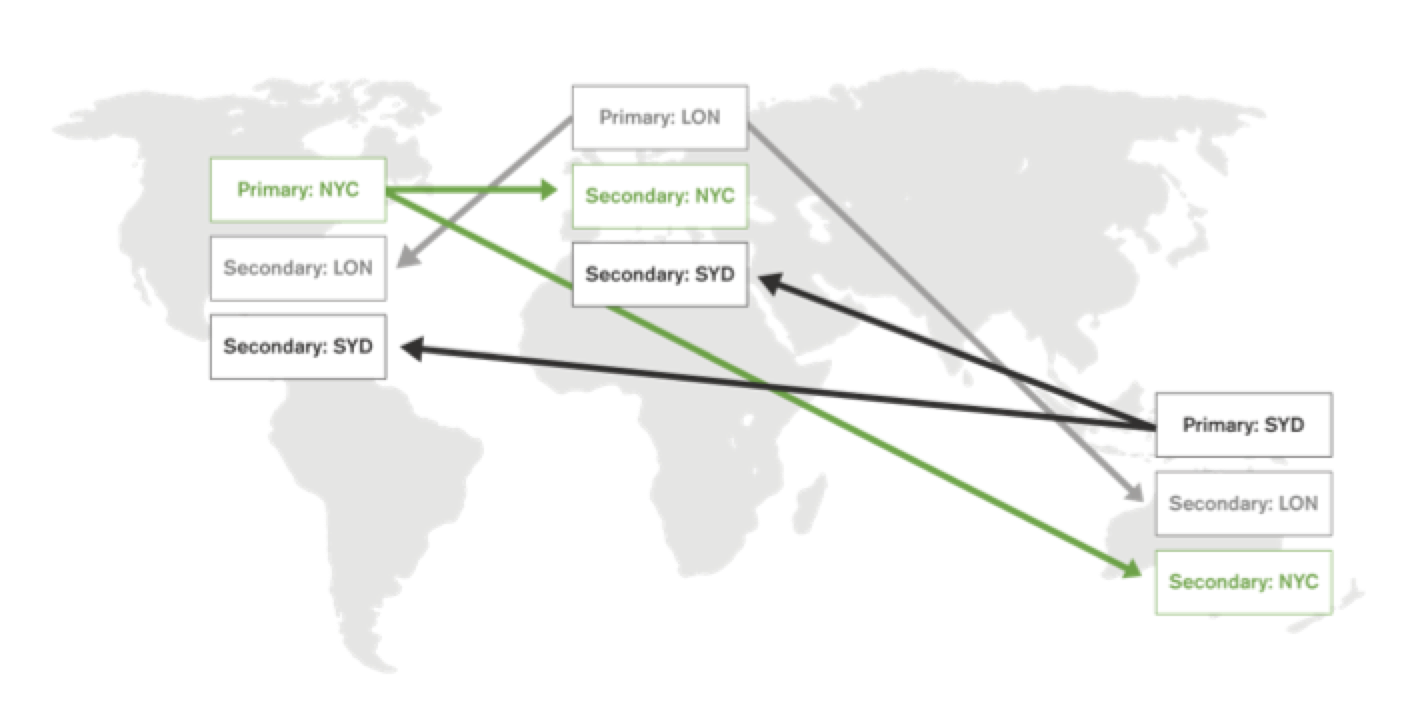
\includegraphics[width=\textwidth]{sources/MongoDB_sharded.png}\cite{db:mongoActiveActiveImage}
	\caption{Regionale Shards mit Replikatgruppen. Sekundärknoten befinden sich für niedrigere Latenzzeiten bei Lesezugriffen in anderen Regionen}
	\label{fig:db:mongoActiveActive}
\end{figure}

\subsubsection{Hochverfügbarkeit}
Für den Anmeldevorgang, die Registrierung und alle Seiten der Anwendung, die einen angemeldeten Nutzer voraussetzen, ist eine Datenbankanbindung zwingend erforderlich.
Sollten diese Dienste ausfallen, ist der Nutzen der Anwendung stark verringert.
Nur statische Seiten, wie die Startseite oder das Impressum, wären in so einem Fall verwendbar.
Dementsprechend bietet sich eine Datenbank mit Hochverfügbarkeit an, um das Risiko eines Ausfalls unserer Plattform so weit wie möglich zu verringern.\\
Um die Erreichbarkeit der Datenbank zu gewährleisten, bietet es sich an, Replikatgruppen zu erstellen.
Eine Replikatgruppe besteht aus mehreren Datenbankprozessen (Knoten), welche den gleichen Datensatz verwalten. \cite{db:mongoReplicaSetMembers}
Sollten durch Hardwarefehler einzelne Knoten ausfallen oder Softwarefehler Knoten dazu zwingen, neu gestartet zu werden, ist die Datenbank, wenn auch mit verringerter Leistung, weiterhin erreichbar.
Die dadurch erreichte Fehlertoleranz schafft Sicherheit und verringert drastisch die Chance, dass die Datenbank komplett ausfällt.\\
In der gewählten Konfiguration hat nur ein Prozess der Replikatgruppe Schreibrechte, um die Konsistenz bei gleichzeitigen Schreibzugriffen zu wahren.
Neben diesem Primärknoten existieren oft mehrere Sekundärknoten, welche die Schreibvorgänge des Primärknotens kopieren und für Lesezugriffe zur Verfügung stehen.\\
Es existieren andere Architekturen mit mehreren Primärknoten, die gleichzeitige Schreibzugriffe erlauben und besondere Herausforderungen bei der Datenkonsistenz stellen (\enquote{Multi-Master-Systeme}).
Diese werden hier nicht betrachtet.

\paragraph{}
PostgreSQL bietet verschiedene Lösungsansätze.
Bei synchronen Lösungen muss ein Schreibauftrag von allen Knoten durchgeführt sein, um als bestätigt zu gelten.
Asynchrone Lösungen erlauben einen Puffer zwischen dem Bestätigen eines Schreibauftrags und dessen Kopie auf andere Knoten.
Dadurch kann das Wechseln zu einem Backupknoten zu Datenverlust führen und Sekundärknoten können bei Lesezugriffen ein leicht veraltetes Ergebnis liefern.
Dafür gewinnt eine asynchrone Lösung an Performanz, da sich die Wartezeit verringert. \cite{db:postgresHighAvailability}\\
Um die Knoten auf dem gleichen Stand zu halten und im Fall eines Ausfalls Daten wiederherstellen zu können, wird ein \textit{Write-Ahead-Log} (WAL) angelegt, welcher unmittelbar nach jedem Commit die Transaktion in einen Transaktionslog schreibt.
Dieser wird dann von anderen Knoten ausgelesen und die Transaktion wird kopiert. \cite{db:postgresWriteAheadLogging}\\
Sollte der Primärknoten ausfallen, muss dies detektiert werden und ein Sekundärknoten mit so wenig Verzögerung wie möglich als neuer Primärknoten ausgewählt werden.
PostgreSQL bietet keine automatische Ausfallsicherung.
Es muss daher eine Drittanbietersoftware verwendet oder ein eigenes Skript geschrieben werden.
Um die Belastung der einzelnen Knoten möglichst gleich zu halten, sollte ein Prozess zur Lastverteilung existieren.
Für die Lastverteilung stehen einige Lösungen von Drittanbietern zur Verfügung.
Nach weitreichender Recherche konnte nicht ermittelt werden, ob PostgreSQL native Lastverteilung anbietet.
Allerdings gibt es verschiedene Projekte, welche Lösungen zur Lastverteilung anbieten. \cite{db:postgresLoadBalancing}


\paragraph{}
Knoten in MongoDBs Replikatgruppen teilen sich gegenseitig durch Ping-Befehle ihren \enquote{Herzschlag} mit, um zu ermitteln, ob ein Knoten ausgefallen ist.
Sollte der Primärknoten \enquote{sterben}, wählen die \enquote{überlebenden} Knoten in einer Abstimmung den nächsten Primärknoten, welcher die Schreibaufträge des vorigen Primärknotens übernimmt.
Der Prozess einer Wahl sollte in der Regel durchschnittlich nicht länger als 12 Sekunden dauern und passiert vollautomatisch \cite{db:mongoElectionTimeout}.
Einem Knoten mit mehr Leistung kann eine höhere Priorität zugewiesen werden, um diesen als präferierten Primärknoten zu definieren \cite{db:mongoElectionPriority}.
Auch eignet es sich, Knoten in anderen Regionen für die Rolle des Primärknoten als unwählbar zu definieren, da sich die Latenz ansonsten drastisch erhöhen würde.
Ein Replikset kann aus maximimal 50 Knoten bestehen, wovon bis zu 7 zum Primärknoten wählbar sind \cite{db:mongoReplicaSetMembersLimit}.
Diese Zahl ist vermutlich groß genug, um einen gleichzeitigen Ausfall aller Knoten aus technischer Sicht nahezu unmöglich zu gestalten, wenn sich die Knoten zusätzlich auf verschiedenen physischen Geräten befinden.\\
In seltenen Fällen kann es vorkommen, dass der Primärknoten ausfällt und vor seinem Ausfall Schreibaufträge bestätigt, diese aber nicht an die Standbyknoten weiterleiten kann. Wenn der frühere Primärknoten der Replikatgruppe wieder beitritt, in diesem Fall als Sekundärknoten, unterscheidet sich dessen Schreibhistorie von der anderer Knoten. Die Historie des früheren Primärknoten wird zurückgerollt und die bestätigten Schreibaufträge sind verloren. 
MongoDB versucht durch verschiedene Techniken, Rollbacks zu vermeiden und erlaubt es unter Verlust von Effizienz, mit Schreibbestätigungen erst zu antworten, wenn der Großteil der Replikatgruppe diese bestätigt hat. \cite{db:mongoRollback}\\
Leseanfragen werden per Standardkonfiguration an den Primärknoten gestellt, um möglichst aktuelle Daten liefern zu können.
Diese Präferenz lässt sich ändern, um den Primärknoten zu entlasten, auf speziell eingerichtete Knoten mit optimisierten Indexen zugreifen zu können, die Latenz zu verringern oder beim Ausfall des Primärknotens weiterhin Lesezugriffe zu ermöglichen. \\
Auch ist eine Wahl zwischen asynchronen und synchronen Operationen möglich.
Dabei sind asynchrone Operationen aufgrund der höheren Performanz die Standardeinstellung.

\paragraph{}
Aus den in diesem Unterkapitel genannten Gründen überzeugt MongoDB im Punkt der Hochverfügbarkeit gegenüber PostgreSQL.
Um PostgreSQL hochverfügbar zu machen, sind einige Anpassungen und Expertenwissen oder Drittanbietersoftware nötig.
MongoDB scheint von der Architektur auf Hochverfügbarkeit ausgerichtet zu sein und liefert Funktionen für eine automatische Ausfallsicherung, welche das System nach kurzer Zeit ohne manuelle Eingriffe wieder voll funktionstüchtig machen.
Es wird vermutet, dass mit MongoDB eine Datenbank eingerichtet werden kann, die mit wenig Aufwand stabil für sehr geringe Ausfallraten sorgen kann.

\subsubsection{Dateiformat}
MongoDB speichert Daten im JSON-Format. 
\enquote{JSON (JavaScript Object Notation) ist ein schlankes Datenaustauschformat, welches für Menschen einfach zu lesen und für Maschinen einfach zu parsen [\dots] ist} \cite{db:json}. 
JSON als semistrukturiertes Dateiformat eignet sich daher gut für Schnittstellendaten.\\
Desweiteren wird im gewählten MERN-Techstack ausschließlich JavaScript verwendet - das JavaScript native Dateiformat JSON ist daher ohne Umwandlungen direkt verwendbar und der Umgang für das Entwicklerteam bereits bekannt.
Dies verringert die Gefahr möglicher Komplikationen und spart Lern- und Programmieraufwand.
Diesen Vorteil besitzt PostgreSQL nicht.
Abfrageergebnisse müssen für die Schnittstelle zuerst in JSON-Dateien geändert werden, was einen zusätzlichen Programmierschritt bedeutet.

\subsubsection{Fazit}
\begin{table}
\centering
\begin{tabularx}{\linewidth}{ |X|X|X| } 
    \hline
    Kriterien & PostgreSQL & MongoDB  \\ 
    \hline
    Lesegeschwindigkeit & Mittel & Hoch \\
    Schreibgeschwindigkeit & Mittel & Langsam - Mittel \\
    Datenstrukturen & Strenges Tabellenschema & Schemafrei durch selbstbeschreibende JSON-Dokumente \\
    Skalierbarkeit & Meist vertikal, horizontal benötigt erweitertes Setup & Meist horizontal, unterstützt nativ Sharding \\
    Hochverfügbarkeit & Replikatgruppen, Lastverteilung und automatische Ausfallsicherung meist über Drittsoftware & native Replikatgruppen und automatische Ausfallsicherung, Lastverteilung bei Wahl eines Sekundärknotens, automatische Wahl des nächsten Primärknotens bei Ausfall \\
    Dateiformat & internes Format, wird bei Abfragen in lesbaren Tabellen ausgegeben & JSON \\
    \hline
\end{tabularx}
\caption{Vergleich PostgreSQL und MongoDB}
\label{db:table:comparisonPostgresMongo}
\end{table}

Es konnte gezeigt werden, dass beide Datenbanken eine ausgereifte Architektur besitzen und sich daher beide gut für Softwareprojekte eignen.
Für dieses Projekt bietet MongoDB einige Vorteile, die sich auf die Entstehungsgeschichte von MongoDB zurückführen lassen.\\
Die 2007 neu gegründete Firma 10Gen, mittlerweile bekannt als MongoDB Inc., benötigte eine Datenbank, welche den Anforderungen ihrer quelloffenen Plattform-as-a-Service Cloud-Architektur gerecht werden würde.
Das Team suchte nach einer Datenbank, die elastisch, skalierbar, einfach zu verwalten und für Entwickler und Anwender einfach zu benutzen ist.
Unzufrieden mit den zu der Zeit auf dem Markt verfügbaren Datenbanksystemen wurde MongoDB, eine dokumentbasierte Datenbank, entwickelt.
Als das Team das Potenzial der Datenbank realisierte, wurde die Idee der Cloud-Plattform eingestellt und die Entwicklung von MongoDB gefördert.\cite{db:mongoHistory}\\
Native Funktionen wie MongoDBs automatische Ausfallsicherung, horizontale Skalierung und Sharding lassen sich wenig Aufwand konfigurieren und skalieren.
Bei der Anwendung werden auf einen komplexen Schreibzugriff vermutlich dutzende bis hunderte Lesezugriffe kommen.
Dementsprechend sorgt die schnellere Lesegeschwindigkeit zu Kosten der Schreibgeschwindigkeit für schnellere Datenbankzugriffe.
Zudem integriert sich das von MongoDB gewählte Dateiformat JSON gut mit der weiteren Architektur des verwendeten MERN-Techstacks.
Aus den genannten Gründen fällt die Wahl der Datenbank für das Projekt auf MongoDB.


\subsection{Schemata}
MongoDB organisiert Daten in Kollektionen.	
Folgende Kollektionen wurden verwendet, um die Daten optimal zu verwalten:

\paragraph{Nutzer}
\begin{table}
    \centering
    \begin{tabularx}{\textwidth}{ |X|X|X| } 
        \hline
        Feld & Beschreibung & Beispiel \\ 
        \hline
        Id & Standardmäßige MongoId & \\
        Benutzername & einzigartiger, öffentlicher Name & MaxMustermann \\ 
        normalisierter Name & Name in Kleinbuchstaben. Wird verwendet, um die Einzigartigkeit von Namen zu gewährleisten & maxmustermann \\ 
        Email & private eMail des Nutzers & mustermann@email.de \\
        Rolle & Gibt an, ob der Nutzer autorisiert ist - Moderatoren und Administratorkonten haben mehr Rechte. Automatisch generiert & Nutzer \\ 
        Geburtsdatum & privates Geburtsdatum des Nutzers & 01.01.2000 \\ 
        Alter & Alter des Nutzers. Wird automatisch mit Geburtsdatum berechnet & 21 \\ 
        Sprachen & Array von Sprachen, die der Nutzer sprechen kann & {[de, en]} \\
        Geschlecht & gesellschaftliches Geschlecht des Nutzers. & Männlich \\ 
        Spielposition & Bis zu 2 Lieblingspositionen des Spielers in League of Legends & {[Mid, Jungle]} \\ 
        Freitext & kurzer Text, in dem der Nutzer sich beschreiben kann. & Ich bin ein toller Nutzer! \\
        Avatar & URI vom Avatarbild des Nutzers & \url{https://<s3-name>.s3.eu-central-1.amazonaws.com/avatars/<UUID>.jpg} \\ 
        Freunde & Array von allen Freunden des Nutzers. Beinhaltet die NutzerID und die ChatID & {[[id1, NutzerID1, ChatID1], [id2, NutzerID2, ChatID2]]}\\ 
        Geblockt & Array von NutzerIDs der Nutzer, die geblockt wurden & {[NutzerID3, NutzerID4]} \\ 
        \hline
    \end{tabularx}
    \caption{Schema Nutzer}
    \label{db:table:nutzer}
\end{table}

Wenn ein Nutzer einen Account erstellt, gibt dieser seine Email-Adresse, den gewünschten Benutzernamen und das gewünschte Passwort an. 
Durch Indexe wird die Einzigartigkeit von eMail und Benutzername geprüft, das Passwort wird aus Sicherheitsgründen in einer separaten Kollektion gespeichert.
Nach der Kontoerstellung kann der Nutzer das Geburtsdatum, die gesprochenen Sprachen, das Geschlecht, die Spielposition und einen Freitext angeben sowie ein Bild hochladen, welches als Avatarbild dient.
Felder wie der normalisierte Name, das Alter und die Rolle werden automatisch generiert.
Im Laufe der Nutzung der Plattform wird der Nutzer andere Spieler als Freunde hinzufügen - diese werden in einer Freundesliste gespeichert.
Auch steht es dem Nutzer frei, Andere zu blockieren - in diesem Fall wird die NutzerID des Blockierten auf die Blockliste hinzugefügt. \\
Privatsphäre und damit die Sicherheit der eigenen Daten stellt einen hohen Stellenwert dar.
Die Anzahl an Daten, die ein Nutzer von sich preisgeben muss, soll so gering wie möglich halten werden.
Die Email-Adresse, das Geburtsdatum und Freundes- und Blockliste sind für andere Nutzer nicht einsehbar.
Bis auf den Benutzernamen, bei welchem es sich um einen Fantasienamen handeln kann, muss eine Person keine Daten öffentlich angeben.

\paragraph{Sprache\\}
Damit Nutzer ihre gesprochenen Sprachen wählen können, bieten wir die Wahl zwischen 187 Sprachen nach ISO 639-1 Norm an.\cite{db:iso639-1}\\

\begin{table}
    \centering
    \begin{tabular}{ |c|c|c| }
    \hline
        Feld & Beschreibung & Beispiel \\
        \hline
        Id & Alpha-2 Code der Sprache & en, de, fr \\
        Name & Englische Schreibweise der Sprache & English, German, French \\
        nativer Name & native Schreibweise der Sprache & English, Deutsch, français \\
        \hline
    \end{tabular}
    \caption{Schema Sprache}
    \label{db:table:sprache}
\end{table}

Standardmäßige Objekt-IDs von MongoDB enthalten einen Zeitstempel und einen inkrementellen Zähler \cite{db:mongoObjectId}.
 Diese Daten sind bei Sprachen - öffentlichen Stammdaten, die sich über einen langen Zeitraum nicht verändern werden - nicht relevant.
Stattdessen wurde der Alpha-2-Code der Sprache als ID gewählt, der in den meisten Fällen auf die Sprache schließen lässt.
Nutzerdokumente referenzieren die Sprache per ID.
Dadurch fällt es leichter, direkt im Nutzerdokument anhand der Sprach-ID zu erkennen, welche Sprachen der Nutzer spricht.
Auch wird das manuelle Kontrollieren von Testfällen hierdurch vereinfacht.
Sprachen können sowohl anhand der englischen Schreibweise als auch der nativen Schreibweise gefunden werden.
Dies erleichtert auch nicht-englischsprachigen Nutzern, ihre Sprache auswählen zu können.

\paragraph{Passwort\\}
\begin{table}
    \centering
    \begin{tabular}{ |c|c| }
        \hline
        Feld & Beschreibung  \\
        \hline
        Id & Standardmäßige MongoId \\
        Passwort & Bcrypt Hash des Passworts bestehend aus Versionsnummer, Komplexität, Salt und Hash \\
        NutzerID & MongoId des zugehörigen Nutzers \\
        \hline
    \end{tabular}
    \caption{Schema Passwort}
    \label{db:table:passwort}
\end{table}

Das Passwort wird nicht im Nutzerdokument gespeichert, da sonst schon kleine Programmierfehler dazu führen könnten, dass normale Nutzer das gehashte Passwort anderer Nutzer ermitteln könnten.
Um dieses Sicherheitsproblem direkt zu eliminieren, wird daher für jedes Passwort ein eigenes, vom Nutzerdokument isoliertes Dokument verwendet.\\
Das Passwort wird durch bcrypt, einem Blowfish-basierten Einweg-Hashalgorithmus, auf der Datenbank als Hash mit Salt gespeichert.
Die Komplexität des Hashes ist frei wählbar und neben Versionsnummer, Salt und dem Hash an sich in der Zeichenkette gespeichtert.\cite{db:bcrypt}\\
Bei der Wahl der Komplexität ist die Sicherheit gegen Rechengeschwindigkeit abzuwägen.
Eine höhere Komplexität erhöht die benötigte Zeit pro Versuch eines Angreifers, das Passwort zu knacken.
Gleichzeitig wird aber auch die Zeit, die unser Server benötigt, um ein neues Passwort zu generieren oder den Anmeldeversuch eines ehrlichen Nutzers zu bestätigen, erhöht.
Eine zu hohe Komplexität kann daher den Server stark verlangsamen und macht Angriffszenarien per (D)DOS ((distributed) denial of service, Überlastung des Servers durch übermäßigen Datenverkehr) gefährlicher, da gezielte Anmeldeversuche viel Last auf dem Server erzeugen.
In Zukunft werden weitere Limitierungen auf Seiten des Backends erstellt, um wiederholte Anmeldeversuche zu bremsen.\\

Zur Verringerung des Erfolges von Brute-Force-Angriffen wird verlangt, dass das Passwort aus mindestens 8 Zeichen, darunter mindestens jeweils 1 Großbuchstabe, 1 Kleinbuchstabe und 1 Ziffer, erstellt wird.
Für mehr Varianz in den Passwörtern sind zudem einige Sonderzeichen erlaubt.
Es besteht eine 1:1-Relation zwischen Passwörtern und Nutzerkonten.

\paragraph{Verhältnis\\}
\begin{table}
    \centering
    \begin{tabular}{ |c|c| }
        \hline
        Feld & Beschreibung  \\
        \hline
        Id & Standardmäßige MongoId \\
        Sender & NutzerID der Person, die den Like/Dislike versendet. \\
        Empfänger &  NutzerID der Person, die den Like/Dislike empfängt. \\
        Status & Gibt an, ob es sich um einen Like oder Dislike handelt. \\
        \hline
    \end{tabular}
    \caption{Schema Verhältnis}
    \label{db:table:like}
\end{table}

Immer wenn ein Nutzer bei der Kontaktsuche angibt, ob er mit einer Person Kontakt aufnehmen oder diesen vermeiden will, wird ein Dokument angelegt. 
Wenn der Nutzer in Kontakt treten möchte, wird zusätzlich geprüft, ob bereits ein Datensatz existiert, bei dem Sender und Empfänger vertauscht sind - ob sich also die Nutzer gegenseitig einen Like gegeben haben. 
In diesem Fall werden beide Datensätze gelöscht und die Nutzer zur Freundesliste des jeweils anderen hinzugefügt und ein Dokument der Kollektion Chat erstellt. 
Die Nutzer können ab dann miteinander kommunizieren. 
Dislikes sorgen dafür, dass ein Kontakt in Zukunft nicht mehr möglich ist.

\paragraph{Chat\\}
\begin{table}
    \centering
    \begin{tabular}{ |c|c| }
        \hline
        Feld & Beschreibung  \\
        \hline
        Id & Standardmäßige MongoId \\
        Teilnehmer & Array von NutzerIDs, die dem Chat beiwohnen. Aktuell maximal 2. \\
        Nachrichten & Array von Nachrichten, die die Nutzer untereinander ausgetauscht haben. \\
        \hline
    \end{tabular}    
    \caption{Schema Chat}
    \label{db:table:chat}
\end{table}

Sollten sich zwei Nutzer befreunden, wird zwischen diesen ein Chat erstellt.
Wenn ein Nutzer die Freundschaft beendet, verlässt dieser gleichzeitig den Chat. 
Mit der gewählten Struktur sind auch Gruppenchats ohne Änderung der Datenbank möglich, falls dies in Zukunft eine erwünschte Funktionalität sein sollte.\\
Um Ressourcen zu sparen, wird bei der Standard-Datenbankabfrage nur die neueste Nachricht geladen.
Diese Abfrage dient für Vorschaubilder des Chats in der Kontaktliste.
Außerdem ist es möglich, durch Pagination (Seitennummerierung) je Abfrage 20 Nachrichten zu erfragen.
Diese Methoden verringern die Serverlast, da in vielen Fällen nicht mehr als die erste Seite der Abfrage relevant ist.\\

\subparagraph{Nachricht\\}
Nachrichten sind eingebettete Dokumente eines Chats.
Sie weisen folgende Datenstruktur auf:

\begin{table}
    \centering
    \begin{tabular}{ |c|c| }
        \hline
        Feld & Beschreibung  \\
        \hline
        Id & Standardmäßige MongoId \\
        Inhalt & Text der Nachricht \\
        Autor & NutzerID des Verfassers der Nachricht \\
        \hline
    \end{tabular}
    \caption{Eingebettetes Schema Nachricht}
    \label{db:table:nachricht}
\end{table}

\subsection{Database-as-a-Service}
Um eine Datenbank selbst zu betreiben fehlt es dem Projekt an fachlichen Kapazitäten und einer Infrastruktur, welche physische Datenbankserver unterstützt.
Es bietet sich daher eine Database-as-a-Service-Lösung (DBaaS) an.\\ 
MongoDB Inc. bietet mit MongoDB Atlas eine DBaaS an, die flexibel auf die Größe und Auslastung des Projektes angepasst werden kann.
Dazu gibt es verschiedene Datenbankstufen, die mit höheren Kosten mehr Rechenleistung und weitere Funktionen erhält.
Zwischen den Stufen kann flexibel gewechselt werden, um den realen Auslastungen gerecht zu werden.
Kostenpflichtige Stufen bieten die Möglichkeit an, Backups einzurichten.
Für höhere Kosten stehen außerdem Werkzeuge zur Verfügung, die Metriken in Echtzeit anzeigen, automatisch archivieren, Empfehlungen zur Leistungsoptimierung erstellen oder langsame Datenbankabfragen zur Diagnose und Optimierung anzeigen.
In der Entwicklungsphase wurde sich für die kostenlose Stufe entschieden, da die Funktionen und Leistung für die Entwicklungsumgebung ausreichen.
Sollte das Produkt auf den Markt gehen, wird auf eine kostengünstigste Stufe gewechselt, um die Option von Backups zu erhalten.
Sollte das Projekt erfolgreich sein und viele Nutzer anziehen, wird flexibel, abhängig von der benötigten Leistung, eine teurere Stufe mit mehr Leistung gewählt.\\
Sowohl die Produktions-, als auch die Entwicklungsumgebung werden als eigene Datenbanken von MongoDB Atlas gehosted (host = Gastgeber, Betrieb der Datenbank durch MongoDB Atlas, Zugriff auf diese über das Internet).
Dies verringert das Risiko von Code, der auf der lokalen Maschine funktioniert, aber auf der Produktionsumgebung Fehler wirft.
Durch die Nutzung gleicher Werkzeuge und gleicher Technologie wird die Werkzeuglücke verringert und dementsprechend die Dev-Prod-Vergleichbarkeit erhöht. \cite{db:devProdParity}

\subsection{Avatarbilder}
Statt Bilddateien für Avatare direkt auf der Datenbank zu speichern, was mit langen Wartezeiten auf die Datenbank einhergehen würde, werden nur die URIs zu den Bildern auf der Datenbank gespeichert.
Für das Speichern der Binärdateien wurde sich für AWS S3 entschieden, einem Speichersystem, welches für BLOB-Dateien (Binary Large OBject) optimiert ist.
Dies nimmt der Datenbank Last ab und erhöht die Anfragegeschwindigkeit bei Lese- und Schreibzugriffen des Avatarbildes.\\
Der S3-Speicher wurde so eingerichtet, dass das Backend Zugriffsrechte zum Erstellen und Löschen von Dateien hat.
Beim Verteilen der Zugriffsrechte wurde nach Minimalprinzip vorgegangen.
Das Backend besitzt nur die minimal nötigen Zugriffsrechte und keine weiteren.
Ein möglicher Angriff verursacht dadurch weniger Schaden, als wenn das Backend alle Zugriffsrechte hätte.\\
Die Datenbank wird mithilfe von GraphQL angesprochen, für S3 hat sich diese Lösung jedoch nicht angeboten.
Für das Hochladen von Profilbildern wurde eine weitere Route im Backend erstellt, bei der mit den npm-Paketen Multer und Multer-S3 kontrolliert wird, ob es sich bei der vom Nutzer hochgeladenen Datei um eine Bilddatei handelt und ob diese eine bestimmte Bildgröße nicht übersteigt.

\subsection*{Fazit}
Mit den gewählten Kollektionen und der Wahl von speziellen Hosts sind wir in der Lage, Nutzern eine Datenbank anzubieten, die eine hohe Erreichbarkeit aufweist, sich leicht an die Auslastung skalieren lässt, personenbezogene Daten geheim hält und ein Maß an Datensicherheit bietet, welches der Größe des Projektes entspricht.
Flexible Datenstrukturen erlauben schnelle Anpassungen des Projektes.
Die Verwendung eines bekannten Dateiformats, welches sich gut für Schnittstellen eignet, sorgt für Zeitersparnisse in der Entwicklung des Frontends und der Datenbankschnittstelle und reduziert somit den Aufwand.
Außerdem werden durch eingebettete Dokumente, Denormalisierung und Seitennummerierung Optimierungen durchgeführt, die als Ziel haben, möglichst schnell Antworten auf Leseanfragen zu bieten.

\newpage
\section{Benutzeroberfläche}\label{kap_benutzeroberflaeche}
\input{chapters/Benutzeroberfläche}

\newpage
\section{Serveranfragen}\label{kap_serveranfragen }
\subsection{GraphQL}
\paragraph{}
GraphQL ist eine Abfragesprache und Server-Laufzeitumgebung für APIs.
Ihre Aufgabe ist es, genau die Daten zu liefern, die anfordert werden, und nicht mehr.
\\
Mit GraphQL sind APIs schnell, flexibel und einfach für Entwickler.
\\ \\
Laut dem 2020 State of the API Report von Postman.com steht GrapQL an fünfter Stelle der spannendsten Technologien für 2021.
% \begin{quote}  {Vgl. u.a. \cite{RH1}} \end{quote}

Im Hinblick auf die Art und Weise, wie Abfragen an den Server mit Hilfe von \\ GraphQL behandelt werden können, sind folgende Aspekte zu beachten.
\\
\begin{quote}
    \textbf{Vorteile}\\

    \begin{itemize}
        \item
              GraphQL-Aufrufe werden in einem einzigen Round Trip gehandhabt. Wir bekommen genau die Daten, die angefragt haben (kein Over-Fetching).

        \item
              Stark definierte Datentypen verringern das Risiko einer Fehlkommunikation zwischen Client und Server.

        \item
              GraphQL ist introspektiv. So können wir eine Liste der verfügbaren Datentypen anfordern. Dies ist ideal für automatisch erstellte Dokumente.

        \item
              Eine Anwendungs-API kann sich mit GraphQL weiterentwickeln, ohne dass bestehende Anfragen beeinträchtigt werden.
        \item
              GraphQL schreibt keine spezifische Anwendungsarchitektur vor. Es kann auf einer vorhandenen REST-API installiert und mit aktuellen API-Management-Tools verwendet werden.
        \item
              Als Alternative zu REST ermöglicht GraphQL Entwicklern die Erstellung von Abfragen zur Extraktion von Daten aus mehreren Quellen mit einem einzigen API-Abfrage.

    \end{itemize}
   
    \textbf{Nachteile}
    \begin{itemize}
        \item
        Für Entwickler, die sich bereits mit REST-APIs auskennen, bedeutet GraphQL weiteren Lernaufwand.
     \item 
     Mit GraphQL verschiebt sich die Funktionalität von Datenabfragen zur Serverseite, was zusätzliche Komplexität für Serverentwickler bedeutet.

\end{itemize}

    \footnote{Vgl. u.a. \cite{RH1}}
\end{quote}

\textbf{Implementierung der Serveranfragen}\\
Alle Abfragen und Mutations wurden in einem separaten Ordner gesammelt.
Damit soll eine saubere Struktur des Codes gewährleistet werden.
Diese wurden für die spätere Verwendung in den React-Komponenten exportiert.

Beim Einloggen in unseren Account werden die entsprechenden Daten geladen, für die zunächst mit Hilfe des ApolloClient Hook useQuery Daten gelesen werden.
In ähnlicher Weise wurde der Schreibprozess mit dem Hook useMutation implementiert.
\\
In diesem Kapitel wird erläutert, wie die beiden oben genannten Abfragen implementiert wurden.


\subsubsection{Leseabfrage} 
\begin{lstlisting}
    export const GET_MY_INFO = gql`
    {
      userSelf {
        _id
        name
        aboutMe
        languages
        gender
        avatar
        ingameRole
        dateOfBirth
        friends { user chat }        
        blocked
      }
    }
  `
//Beispiel einer Abfrage
\end{lstlisting}
Der obige Code zeigt die Felder der userSelf-Anfrage.
Es ist auch möglich, über GraphQL Playground selbst die automatisch generierte Dokumentation einzusehen. 
Dort seiht man alle verfügbaren Felder und deren Datentyp.
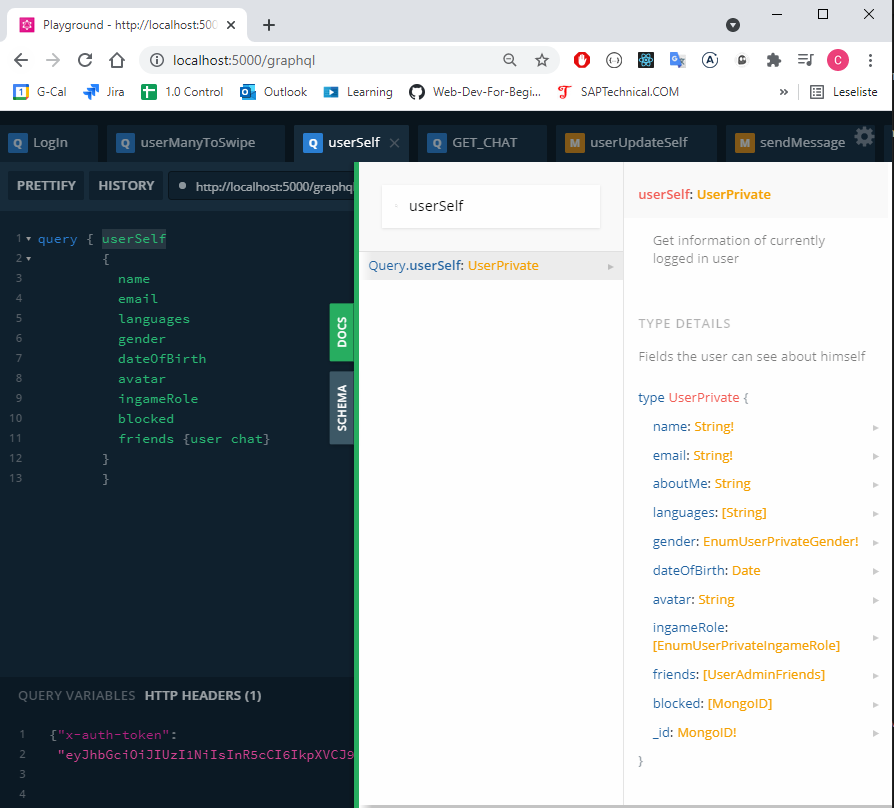
\includegraphics[scale=0.60]{GraphQL_Playground}

\newpage
\textbf{Apollo Client}\\
%Warum haben wir uns dafür entschieden?
Nachdem eine Abfrage exportiert wurde, ist sie bereit, in einer React-Komponente importiert \\ 
und angewendet zu werden.

\begin{lstlisting}
import { GET_MY_INFO } from "./GraphQL/Queries"
import { useQuery } from "@apollo/client"

const { loading, error, data } = useQuery(
GET_MY_INFO,
ContextHeader(token),
)
//Code-Auszug in frontend/src/App.js

\end{lstlisting}
Die Konstante ContextHeader enthält das Token in der Struktur, die erforderlich ist, um die Abfrage nur dann stellen zu können, wenn der Benutzer dazu berechtigt ist.
\\
Sollte das Token undefined, null oder ungültig sein, wird der Server ein Fehler zurückgegeben.
\\ 
Der useQuery Hook liefert ein Ergebnisobjekt, welches eine der folgenden Optionen zurückgibt.
\\
\textbf{loading:}\\
Ein boolescher Wert, der angibt, ob die Abfrage in Bearbeitung ist.
Wenn loading true ist, ist die Anfrage noch nicht abgeschlossen. Typischerweise kann diese Information verwendet werden, um einen Lade-Spinner anzuzeigen.
\\
\textbf{error:}\\
Ein Laufzeitfehler mit den Eigenschaften von GraphQL Errors und network Error.
Dieses enthält Informationen darüber, was bei der Abfrage schief gelaufen ist.
\\
\textbf{date:}\\
Ein Objekt, das das Ergebnis der GraphQL-Abfrage enthält.
\\Es enthält die tatsächlichen Daten vom Server.
\\

AUCH MUTATIONS ZEIGEN\dots
\newpage
\subsection{Axios}
Zusätzlich zu den GraphQL-Abfragen, wurde eine Post-Anfrage mit Axios bereitgestellt.
Mit dieser war es möglich, Bilder auf die S3 Speicher von AWS hochzuladen.

\begin{quote}
Axios ist ein Promise-basierter HTTP-Client für node.js und den browser. Er ist isomorphisch (= kann auf dem server und im browser verwendet weden). Auf der Server-Seite wir das modul http verwendet, während im Browser XMLHttpRequests (ajax) ausgeführt werden.
\end{quote}

\begin{lstlisting}
    function disableBtn() {
        const uploadBtn = document.getElementById("uploadBtn")
        uploadBtn.disabled = true
        uploadBtn.style.background = "#000000"
      }
    
      function fileUploadHandler() {
        errored ? 
         disableBtn()
         /*
        Tritt ein Fehler auf, wird die Abfrage nicht gesendet und der Knopf deaktiviert 
        Ein Fehler tritt auf, wenn die Datei zu gross ist oder oder wenn sie ein ungueltiges  Format hat
        */
        :
        console.log("uploading pic...", file?.name)
        const fd = new FormData()
        /* avatar ist der Name der Datei, die hochgeladen wird
          file ist der zu sendende  Wert */
        fd.append("avatar", file)  
    
        axios
          .post(urlAvatar, fd, {
            headers: {
              "x-auth-token": TOKEN,
            },
          })
          .then((res) => {
            setState((state) => ({ ...state, avatar: res?.data?.location }))    
            //In location finden wir die URL fuer das gerade hochgeladende Bild 
          })
      }\end{lstlisting}

Das HTML-Eingabefeld "input" wurde folgendermaße definiert.
\begin{lstlisting}
    <input type="file" onChange={fileSelectedHandler} />
\end{lstlisting}


Das Format der hochzuladenden Dateien wurde limitiert, damit nur zulässige Dateien an den Server gesendet werden.
\begin{lstlisting}
    const admittedImageFormats = ["png", "jpg", "jpeg"]
\end{lstlisting}

Die Größe der hochzuladenden Datei wurde um 1Mb abgegrenzt.
Durch die Eigenschaft „size“ der ausgewählten Datei konnten wir auf die Größe der Datei zugreifen.
\begin{lstlisting}
    const imageSize = e.target.files[0].size
\end{lstlisting}

\newpage
\section{Qualitätssicherung }\label{kap_QS}
\input{chapters/Qualitätssicherung}

%Temporär, danach sollten wir das Package glossaries benutzen
\newpage
\section{Glossar}\label{kap_glossar}
%\newglossaryentry{kiln}
%{
 % name=kiln,
  %description={German: Brennofen (m.);\\Français: fourneau (m.)},
  %plural=kilns
%}

%Make Glossary properly...
%\acrodef{VB}{Visula Basic}

\textbf{Hooks:}\\
...
\textbf{Framework:}\\
...
\textbf{JSX:}\\
Es heißt JSX und ist eine Syntaxerweiterung für JavaScript. Wir empfehlen, sie mit React zu verwenden, um zu beschreiben, wie die Benutzeroberfläche aussehen soll. JSX erinnert vielleicht an eine Template-Sprache, aber es verfügt über die volle Leistungsfähigkeit von JavaScript. JSX erzeugt React-"Elemente"

\textbf{Under-Fetching:}\\

\textbf{Over-Fetching:}\\
Empfang von überschüssigen Daten durch eine Abfrage.
%Reference https://jwt.io/

\textbf{Web Token:}\\
JSON-Web-Tokens sind eine dem Industriestandard RFC 7519 entsprechende Methode zur sicheren Darstellung von Forderungen zwischen zwei Parteien.

\textbf{undefined:}\\
Eine Variable, der kein Wert zugewiesen wurde oder die überhaupt nicht deklariert wurde (nicht deklariert, existiert nicht), ist undefiniert. Eine Methode oder Anweisung gibt auch undefiniert zurück, wenn der ausgewerteten Variablen kein Wert zugewiesen wurde. Eine Funktion gibt undefiniert zurück, wenn kein Wert zurückgegeben wurde.

\textbf{FormData:}\\
Die FormData-Schnittstelle bietet eine einfache Möglichkeit, eine Reihe von Schlüssel/Wert-Paaren zu erstellen, die die Felder eines Formulars und ihre Werte darstellen und mit der XMLHttpRequest.send()-Methode einfach gesendet werden können.

\textbf{Akronyme:}\\

{AWS}{Amazon Web Services}\\
{DOM}{Document Object Model}\\
{API}{Application Programming Interface}\\



\newpage
\section{Zusammenfassung und Ausblick}\label{kap_zusammfAusbl}
%\input{}
TEXT MUSS KONTROLIERT WERDEN...\\
Es hat sich gezeigt, dass moderne Entwicklungswerkzeuge für JavaScript auch ohne umfassende Kenntnisse der Softwareentwicklung zugänglich sind.

Das Ziel, eine echte Plattform zu schaffen, wurde im Zeitraum von Mai 2021 bis Mitte August 2021 erreicht.

Das heißt, ein Team von zwei Studenten mit grundlegenden Programmierkenntnissen war in der Lage, eine funktionelle Plattform zu schaffen, die die Registrierung, die Anmeldung der Benutzer, die Verwaltung von persönlichen Daten, die Interaktion mit anderen Benutzern auf der Grundlage ihrer Präferenzen umfasst und einen auf Textnachrichten basierenden Kommunikationskanal.

%<MERKKASTEN> (für die eigene Verwendung bitte entfernen
\vspace{1cm}
\begin{tcolorbox}[title={Inhalte der \textit{Zusammenfassung und Ausblick}}]
  Das Kapitel \textit{Zusammenfassung und Ausblick} enthält folgende formale Aspekte\footnote{Vgl. \cite{BBoJ},S. 6}:
  \begin{itemize}
    \item Kapitelweise Kurzdarstellung der Inhalte (inklusive Referenzierung auf die Kapitelnummerierung) => Nach dem Motto: \textit{Was wurde wo beschrieben?}
    \item Kurzdarstellung \textit{Problem – Lösungsweg – Ergebnisse}
    \item Rückkopplung auf die Einleitung: Wurde die Zielstellung der Arbeit und die Fragestellung zufriedenstellend beantwortet?
    \item Kritische Bewertung (sofern nicht bereits im Hauptteil geschehen)
    \item Offene Probleme
    \item Richtung der zukünftigen/möglichen Arbeiten
    \item Erläuterung, warum welche Aspekte in der Arbeit nicht erläutert wurden
  \end{itemize}
\end{tcolorbox}

\section{Literaturverzeichnis}\label{kap_literaturverzeichnis}
    % INFO: Biblatex -Ausgabe des  
  % Literaturverzeichnisses (Beispiele):   
  % - \printbibliography => Ausgabe ALLER 
  %   Einträge
  % - \printbibliography[nottype=online]
  %   => Ausgabe der Einträge, bis auf die
  %      "Online"-Einträge
  % - \printbibliography[type=online]     
  %   => Ausgabe nur der "Online"-Einträge  
   %\printbibliography

  
  % Literaturverzeichnis
   % INFO: Referenzieren auf das Literaturverzeichnis:
   %
   % Befehl: \cite{refmarke}
   % 
   % "refmarke" ist die Angabe in den geschweiften Klammern bei 
   % \bibitem[]{refmarke}. 
   \newpage
    \thispagestyle{empty}
   \section{Quellenverzeichnis}
     \subsection{Literatur}
     \renewcommand{\refname}{} % Literaturverzeichnis ohne Bezeichnung
     % Literaturverzeichnis
     \begin{thebibliography}{SW11} % 2. {...} => Hier die größte /breiteste Nummer (z.B. 99) oder Kurzbeleg angeben.
       \bibitem{SW11} Stickel-Wolf, Christine; Wolf, Joachim (2011): Wissenschaftliches Lernen und Lerntechniken. Erfolgreich studieren–-gewusst wie!. Wiesbaden: Gabler. 
        % TODO cite correctly
       \bibitem{PG01} Seite 51 Zeile 5-6 https://www.researchgate.net/profile/Ciprian-Octavian-Truica/publication/264416935_Asynchronous_Replication_in_Microsoft_SQL_Server_PostgreSQL_and_MySQL/links/53dbe6160cf216e4210c0375/Asynchronous-Replication-in-Microsoft-SQL-Server-PostgreSQL-and-MySQL.pdf
       \bibitem{DB01} Scalability Databases https://ieeexplore.ieee.org/abstract/document/7369245
      \end{thebibliography} 
          
     \subsection{Internetquellen}
     \begin{thebibliography}{HR08} % 2. {...} => Hier die größte/breiteste Nummer (z.B. 99) oder Kurzbeleg angeben.
       \bibitem{BBoJ}Bertelsmeier, Birgit (o. J.): Tipps zum Schrei\-b\-en ei\-n\-er Ab\-sch\-luss\-ar\-beit. Fach\-hoch\-schu\-le Köln-Campus Gummersbach, Institut für Informatik. \url{http://lwibs01.gm.fh-koeln.de/blogs/bertelsmeier/files/2008/05/abschlussarbeitsbetreuung.pdf} (29.10.2013).
        \bibitem{HR08} Halfmann, Marion; Rühmann, Hans (2008): Merkblatt zur Anfertigung von Projekt-, Bachelor-, Master- und Diplomarbeiten der Fakultät 10. Fachhochschule Köln-Campus Gummersbach.\url{http://www.f10.fh-koeln.de/imperia/md/content/pdfs/studium/tipps/anleitungda270108.pdf} (29.10.2013).
        \bibitem{V01} Offizielle Vue-Website: Vergleich zwischen Vue, React und Angular. \url{https://vuejs.org/v2/guide/comparison.html#Preact-and-Other-React-Like-Libraries} (unbekannte Veröffentlichung).
        \bibitem{R01}Offizielle React-Website: React Hooks. \url{https://reactjs.org/docs/hooks-faq.html#which-versions-of-react-include-hooks}
        \bibitem{A01}Offizielle Website Apollo für React. \url{https://www.apollographql.com/docs/react/}
        \bibitem{SO01}StackOverFlow: Developer Survey 2021. \url{https://insights.stackoverflow.com/survey/2021#section-most-popular-technologies-web-frameworks}
        \bibitem{EE1}Elad Elrom: React and Libraries. \url{https://link.springer.com/content/pdf/10.1007%2F978-1-4842-6696-0.pdf}
        \bibitem{SS1}Stoyan Stefanov: Durchstarten mit React. \url{https://content-select.com/media/moz_viewer/5d5fc360-478c-4038-ac17-246bb0dd2d03/language:de}
        \bibitem{RH1}Red Hat: Was ist GraphQL? \url{https://www.redhat.com/de/topics/api/what-is-graphql}
        \bibitem{PM1}Postman: 2020 State of the API Report \url{https://www.postman.com/state-of-api/the-future-of-apis/#the-future-of-apis}
        \bibitem{AX1}Offizielle Website Axios \url{https://axios-http.com/}

        \bibitem{PG11}Offizielle Webseite PostgreSQL \url{https://www.postgresql.org/}
        \bibitem{PG12}PostgreSQL: Warum sollte man PostgreSQL verwenden? \url{https://www.postgresql.org/about/}
        \bibitem{PG13}Stackshare: Wer benutzt PostgreSQL? \url{https://stackshare.io/postgresql}

        \bibitem{MG1}Offizielle Webseite MongoDB \url{https://www.mongodb.com/de-de}
        \bibitem{MG2}Sharding \url{https://docs.mongodb.com/manual/sharding/}
        \bibitem{MG3}Replizierung \url{https://docs.mongodb.com/manual/replication/}
        \bibitem{MG2}NoSQL Erklärt \url{https://www.mongodb.com/de-de/nosql-explained}
        \bibitem{JSON1}Einführung in JSON \url{https://www.json.org/json-de.html}

        \bibitem{12FA1}The Twelve-Factor-App: X.Dev-Prod-Vergleichbarkeit \url{https://12factor.net/de/}


     \end{thebibliography}
% Anhang
\newpage
\setcounter{section}{0} % Nummerierung der Gliederungsebene "section" auf 0 setzen
\renewcommand*\thesection{\Alph{section}} % Nummerierungsart für die Gliederungsebene "section"
% auf Großbuchstaben setzen
\section{Anhang}\label{anhang}
\subsection{Aufwandsverteilung}\label{subsec_UabsAnhang}
Hier zeigen wir, wie die Aufgaben unter den Autoren des Projekts verteilt wurden.
TABELLE/Bild KOMMT...

\subsection{Verwendete Technologien und Werkzeuge}\label{subsec_UabsAnhang}
NodeJS
\\
React
\\
Bootstrap
\\
GitHub
\\
Cypress
\\
VSC
\\
Heroku
\\
LaTeX
\\
Cypress

\newpage

% Erklärung über die selbständige Abfassung der Arbeit
\pagestyle{empty}
\section*{Erklärung über die selbständige\\Abfassung der Arbeit} % \section*{...}: das *-Symbol erlaubt, dass dieser
% Gliederungspunkt nicht ins Inhaltsverzeichnis aufgenommen wird
\addcontentsline{toc}{section}{Erklärung über die selbständige Abfassung der Arbeit}
Ich versichere, die von mir vorgelegte Arbeit selbständig verfasst zu haben.
Alle Stellen, die wörtlich oder sinngemäß aus veröffentlichten oder nicht veröffentlichten Arbeiten anderer entnommen sind,
habe ich als entnommen kenntlich gemacht.\\
Sämtliche Quellen und Hilfsmittel, die ich für die Arbeit benutzt habe, sind
angegeben. Die Arbeit hat mit gleichem Inhalt bzw. in wesentlichen Teilen noch keiner anderen Prüfungsbehörde vorgelegen.\\\\
\begin{tabular}{cp{7cm}}
                                    &             \\
                                    &             \\ \hline
  \small (Ort, Datum, Unterschrift) & \normalsize \\
\end{tabular}

%<MERKKASTEN> (für die eigene Verwendung bitte entfernen
\vspace{1cm}
\begin{tcolorbox}[title={Hinweise zur obigen \textit{Erklärung}}]
  \begin{itemize}
    \item Bitte verwenden Sie nur die Erklärung, die Ihnen Ihr \textbf{Prüfungsservice} vorgibt. Ansonsten könnte es passieren, dass Ihre Abschlussarbeit nicht angenommen wird. Fragen Sie im Zweifelsfalle bei Ihrem Prüfungsservice nach.
    \item Sie müssen \textbf{alle abzugebende Exemplare} Ihrer Abschlussarbeit unterzeichnen. Sonst wird die Abschlussarbeit nicht akzeptiert.
    \item Ein \textbf{Verstoß} gegen die unterzeichnete \textit{Erklärung} kann u.\,a. die Aberkennung Ihres akademischen Titels zur Folge haben.
  \end{itemize}
\end{tcolorbox}
%</MERKKASTEN>

\newpage
% Unbeschriftetes Abschlussblatt (Leere Seite)
\thispagestyle{empty}
\input{leereSeite}



\end{document}

